%%%%%%%%%%%%%%%%%%%%%%%%%%%%%%%%%%%%%%%%%
% Beamer Presentation
% LaTeX Template
% Version 1.0 (10/11/12)
%
% This template has been downloaded from:
% http://www.LaTeXTemplates.com
%
% License:
% CC BY-NC-SA 3.0 (http://creativecommons.org/licenses/by-nc-sa/3.0/)
%
%%%%%%%%%%%%%%%%%%%%%%%%%%%%%%%%%%%%%%%%%

%----------------------------------------------------------------------------------------
%	PACKAGES AND THEMES
%----------------------------------------------------------------------------------------

\documentclass{beamer}

\mode<presentation> {

% The Beamer class comes with a number of default slide themes
% which change the colors and layouts of slides. Below this is a list
% of all the themes, uncomment each in turn to see what they look like.

%\usetheme{default}
%\usetheme{AnnArbor}
%\usetheme{Antibes}
%\usetheme{Bergen}
%\usetheme{Berkeley}
%\usetheme{Berlin}
%\usetheme{Boadilla}
%\usetheme{CambridgeUS}
%\usetheme{Copenhagen}
%\usetheme{Darmstadt}
%\usetheme{Dresden}
%\usetheme{Frankfurt}
%\usetheme{Goettingen}
%\usetheme{Hannover}
%\usetheme{Ilmenau}
%\usetheme{JuanLesPins}
%\usetheme{Luebeck}
\usetheme{Madrid}
%\usetheme{Malmoe}
%\usetheme{Marburg}
%\usetheme{Montpellier}
%\usetheme{PaloAlto}
%\usetheme{Pittsburgh}
%\usetheme{Rochester}
%\usetheme{Singapore}
%\usetheme{Szeged}
%\usetheme{Warsaw}

% As well as themes, the Beamer class has a number of color themes
% for any slide theme. Uncomment each of these in turn to see how it
% changes the colors of your current slide theme.

%\usecolortheme{albatross}
%\usecolortheme{beaver}
%\usecolortheme{beetle}
%\usecolortheme{crane}
%\usecolortheme{dolphin}
%\usecolortheme{dove}
%\usecolortheme{fly}
%\usecolortheme{lily}
%\usecolortheme{orchid}
%\usecolortheme{rose}
%\usecolortheme{seagull}
%\usecolortheme{seahorse}
%\usecolortheme{whale}
%\usecolortheme{wolverine}

%\setbeamertemplate{footline} % To remove the footer line in all slides uncomment this line
%\setbeamertemplate{footline}[page number] % To replace the footer line in all slides with a simple slide count uncomment this line

%\setbeamertemplate{navigation symbols}{} % To remove the navigation symbols from the bottom of all slides uncomment this line
}

\usepackage{graphicx} % Allows including images
\usepackage{booktabs} % Allows the use of \toprule, \midrule and \bottomrule in tables

%----------------------------------------------------------------------------------------
%	TITLE PAGE
%----------------------------------------------------------------------------------------

\title[Distributed Map Reduce]{Distributed Map Reduce} % The short title appears at the bottom of every slide, the full title is only on the title page

\author{A. Emirhan Karag\"{u}l - M. Hakan Kurto\u{g}lu} % Your name
\institute[] % Your institution as it will appear on the bottom of every slide, may be shorthand to save space
{
Bogazici University \\ % Your institution for the title page
\medskip
%\textit{john@smith.com} % Your email address
}
\date{December 24, 2018} % Date, can be changed to a custom date

\begin{document}

\begin{frame}
\titlepage % Print the title page as the first slide
\end{frame}

%----------------------------------------------------------------------------------------
%	PRESENTATION SLIDES
%----------------------------------------------------------------------------------------

%------------------------------------------------
%\section{First Section} % Sections can be created in order to organize your presentation into discrete blocks, all sections and subsections are automatically printed in the table of contents as an overview of the talk
%------------------------------------------------

%\subsection{Subsection Example} % A subsection can be created just before a set of slides with a common theme to further break down your presentation into chunks

%------------------------------------------------

\begin{frame}
\frametitle{Problem Definition}
\begin{columns}[c]
\column{.5\textwidth} % Left column and width
\begin{itemize}
\item Lots of idle resources are present in the office network 
\item Not enough local computing power 
\item Overhead of using cloud computing 
\item Need for a neat CLI tool for remote execution in LAN 
\item Simple as spinning threads
\end{itemize}
\column{.5\textwidth} % Left column and width
\begin{figure}
    \centering
    
\includegraphics[width=0.75\linewidth]{iceberg.jpeg}
\end{figure}
\end{columns}
\end{frame}

%------------------------------------------------
\begin{frame}{Implementation Details}
\quad Client\\
\begin{itemize}
    \item Backbones of the office
    \item Potential to leverage parallel execution over LAN
    \item Send discoveries via UDP Broadcast
    \item Scatter operations
    \item Gather results
\end{itemize}
\end{frame}
%------------------------------------------------

\begin{frame}{Implementation Details}
\quad Server \\
\begin{itemize}
    \item Idle computers in the office
    \item Computers that are being used for excel only by our coworkers :)
    \item Waiting for discoveries (UDP)
    \item Respond to script offers with their status
    \item Execute script to read contents and send back
    \item Times out on reaching time resource allocated 
\end{itemize}
\end{frame}

%------------------------------------------------

\begin{frame}
\frametitle{Proposed Solution}
\begin{figure}
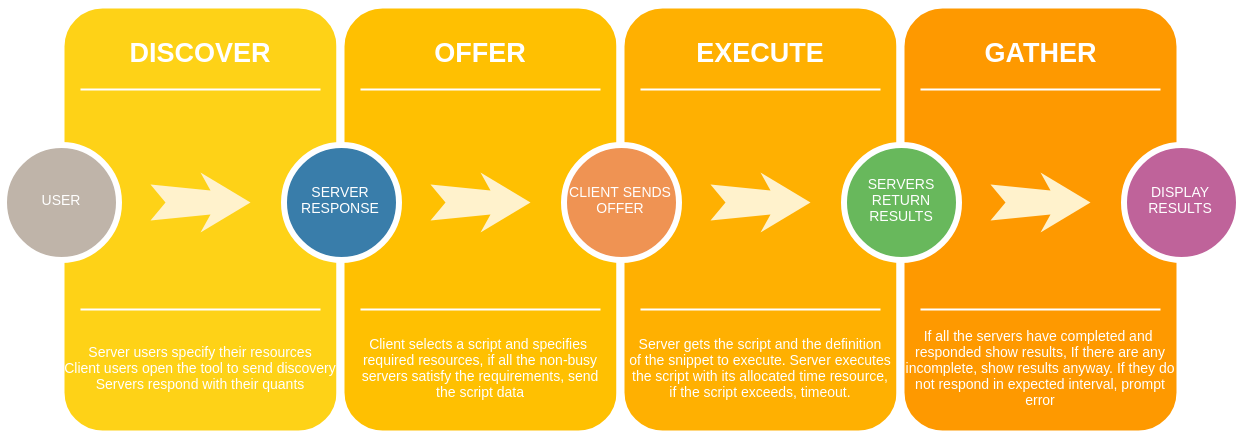
\includegraphics[width=1\linewidth]{flow.png}
\end{figure}
\end{frame}

%------------------------------------------------

%------------------------------------------------

\begin{frame}
\frametitle{Example }
\begin{columns}[c] % The "c" option specifies centered vertical alignment while the "t" option is used for top vertical alignment

\column{.5\textwidth} % Left column and width
\begin{figure}
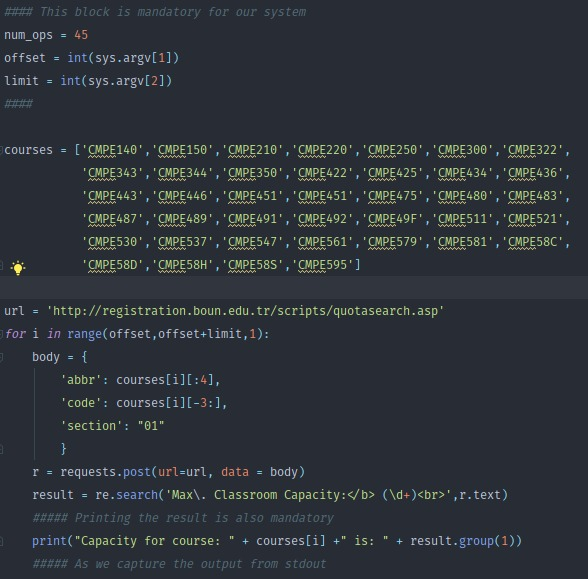
\includegraphics[width=1\linewidth]{example_script.jpeg}
\caption{Example script}
\end{figure}

\column{.5\textwidth} % Right column and width
\begin{figure}
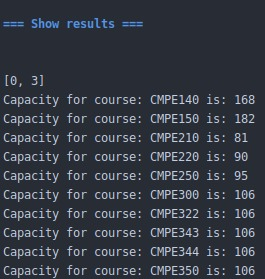
\includegraphics[width=0.93\linewidth]{example_results.jpeg}
\caption{Example result}
\end{figure}
\end{columns}
\end{frame}

%------------------------------------------------

\begin{frame}
\Huge{\centerline{Thank You}}
\Huge{\centerline{For Your Attention!}}
\end{frame}

%------------------------------------------------
\end{document}